
\mysection[black]{2. Computer Graphics}


\mysubsection{2.1 Graphics Pipeline}

\begin{enumerate}[leftmargin = *,noitemsep]
\item \textbf{Modeling transform}: From object to world-space 
\item \textbf{Viewing transform}: From world to camera-space
\item \textbf{Primitive processing}: Output primitives from trans formed vertcies
\item \textbf{3D clipping}: Remove primitives outside frustum
\item \textbf{Projection to screen-space}
\item \textbf{Scan conversion}: Discretize continuous primitives, interpolate attributes at covered samples
\item \textbf{Lighting, shading, texturing}: Compute colors 
\item \textbf{Occlusion handling}: Update color (e.g. z-buffers) 
\item \textbf{Display}
\end{enumerate}
To achieve interactivity, every step has to be reversible.\\
\textbf{Visualisation Pipeline}: Mapping thematic data (i.e. visualisation of statistics on a map) via attributed geometry into images. Has the following steps: Data Generation, Data Filtering, Visualisation Tools, Rendering, Display.
\textbf{Contemporary Pipeline}: CPU, Vector processing (pervertex ops, transforms, lighting flow control), Rasterization, Fragment processing (per-fragment ops, shading, texturing, blending), Display.\\
\textbf{Intercept Theorem}: 
\begin{center}


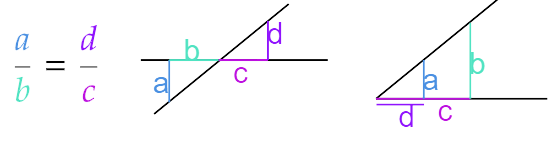
\includegraphics[scale = 0.5]{../images/intercept_theorem.png} 
\end{center}





\mysubsection{2.2 Light \& Colors}
Light is mixture of many wavelengths. Consider $P(\lambda)$ as intensity at wavelength $\lambda$. Humans project inf. dimens. to 3D color (RGB). CIE experiment: some colors are not comb. of RGB. (neg. red needed)

\begin{multicols}{2}
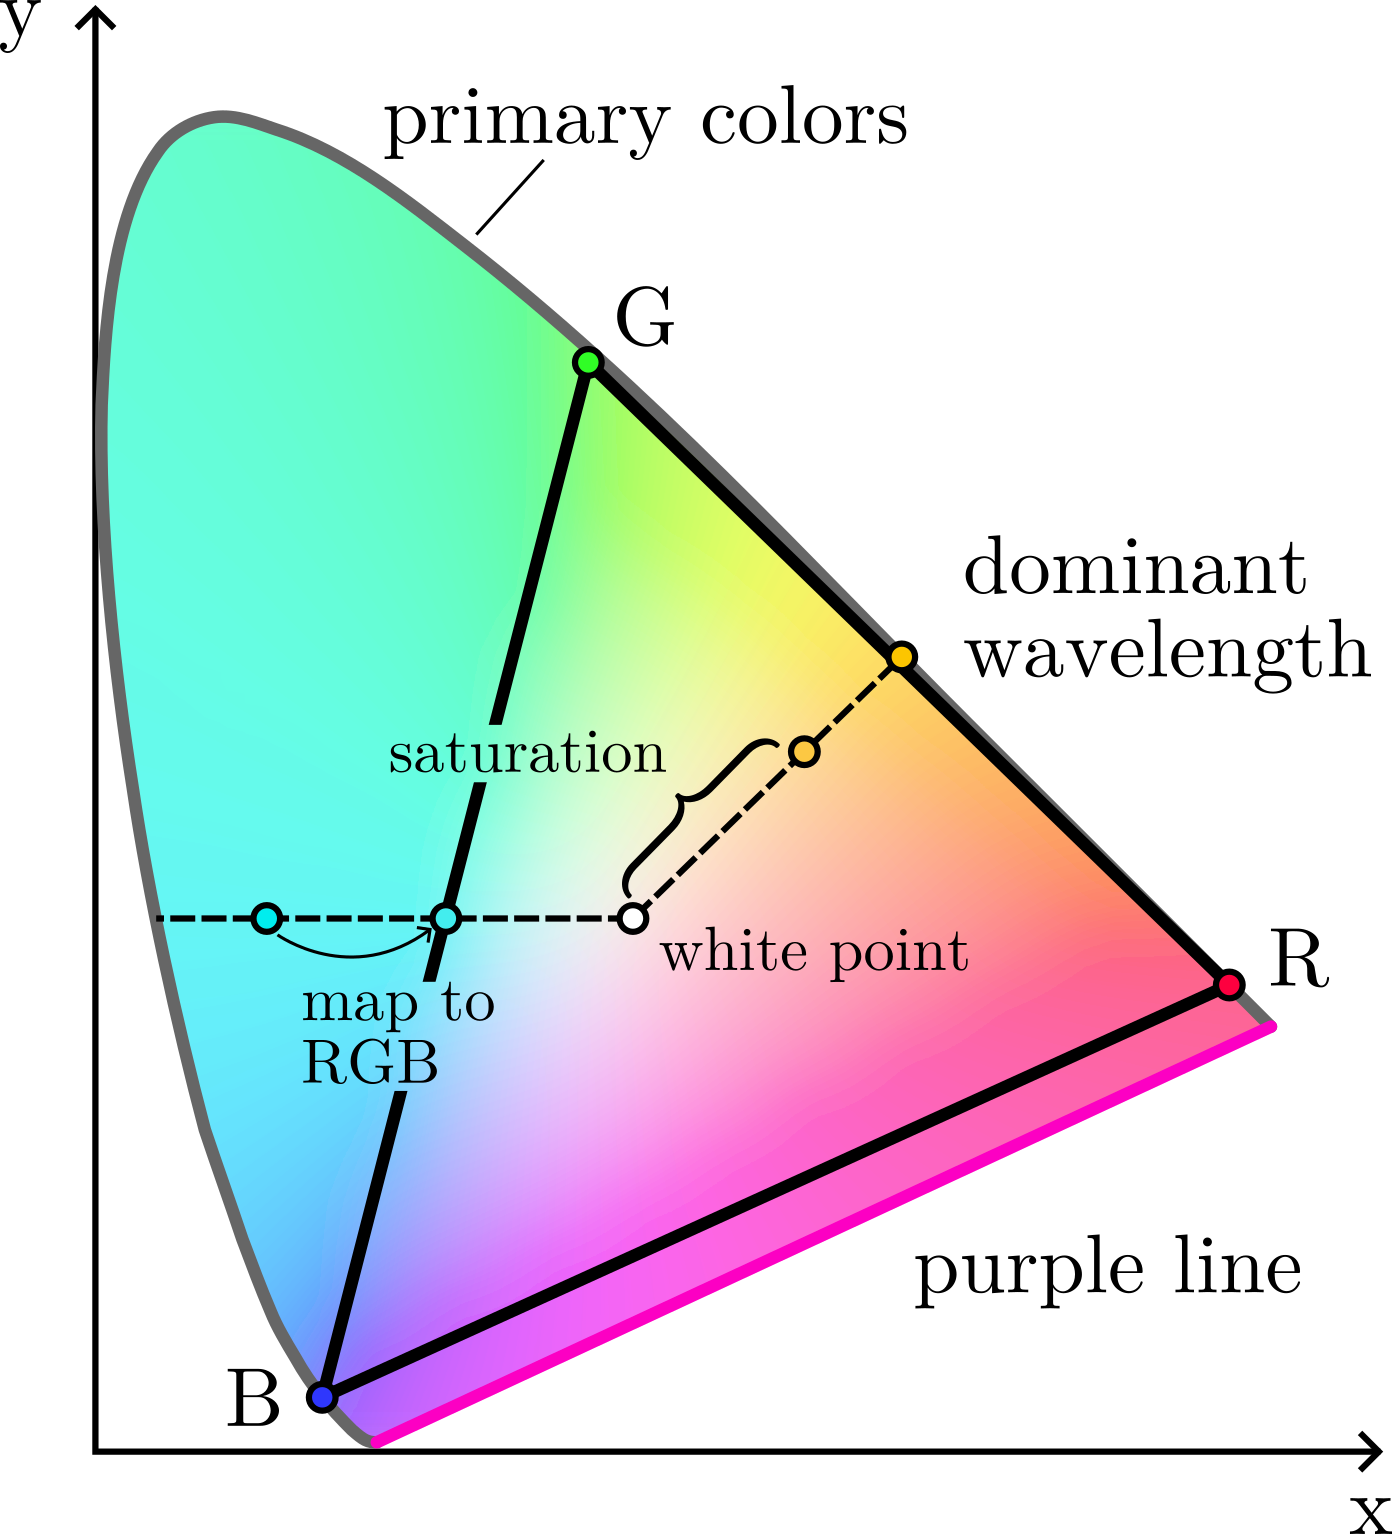
\includegraphics[width = \linewidth]{../images/ciergb.png} 
\columnbreak



\textbf{Mixing Colors}: Mixing 3 lin. ind. primaries in the CIE-Chart: all colors inside/on spanning triangle creatable\\
\textbf{Isoline Sat.}: Parallel to round border:\\
\textbf{Mac Adams Ellipses}: Quantifies how humans perceive diff. in color, not uniform across the spectrum.  


\end{multicols}


\BDEF{Color Spaces}{
\textbf{RGB }(useful for displays, RGB colors specified) \\
\textbf{CIE XYZ}: Change of basis to a
 neg. comp.\\
\textbf{CIE xyY}: Chromaticity (color) $(x, y)$ derived by normalizing XYZ color components: $x=\frac{X}{X+Y+Z}, y=$ $\frac{Y}{X+Y+Z}$. Y is brightness. \\
\textbf{CIE RGB}: (435.8, 546.1, 700.0 nm ). Linear combination span triangle, the Color Gamut.\\
\textbf{CMY}: inverse (subtr.) to RGB. CMY = $1-\mathrm{RGB}$.\\
\textbf{YIQ}: Luminance Y, In-phase I (orange-blue), Quadrature Q (purple-green).

$
\left(\begin{array}{c}
Y \\
I \\
Q
\end{array}\right)=\left(\begin{array}{ccc}
0.299 & 0.587 & 0.114 \\
0.596 & -0.275 & -0.321 \\
0.212 & -0.523 & 0.311
\end{array}\right)\left(\begin{array}{l}
R \\
G \\
B
\end{array}\right)
$


\textbf{HSV}: hue (base color), saturation (purity of color), value / lightness / brightness (intuitive)\\
\textbf{CIELAB / CIELUV}: Correct CIE chart colors to adjust for perceived "distance" betw. colors, nonlinear warp. MacAdams ellipses nearly circular.}


\mysubsection{2.3 Transformations}


\textbf{Homogeneous Coordinates}: Can represent affine maps (translation) with mat.-mul. Add dimension, project vertices $(x\,y\,z)^T$ onto $(\frac{x}{w}\,\frac{y}{w}\,\frac{z}{w},w)^T = (x\, y \, z \, w)^T$. Scale Invariant, vector space

\BEX{}{

\begin{tabular}{lllll}
Trans. &  Scale &  Rot(x) \\
$
\left(
\begin{smallmatrix}
1 & 0 & 0 & t_x\\ 
0 & 1 & 0 & t_y\\ 
0 & 0 & 1 & t_z \\
0 & 0 & 0 & 1 \\
\end{smallmatrix}
\right)$ &
$
\left(
\begin{smallmatrix}
s_x & 0 & 0 & 0\\ 
0 & s_y & 0 & 0\\ 
0 & 0 & s_z & 0 \\
0 & 0 & 0 & 1 \\
\end{smallmatrix}
\right)$ &
$
\left(
\begin{smallmatrix}
1 & 0 & 0 & 0\\ 
0 & \cos \phi & -\sin \phi & 0\\ 
0 & \sin \phi & \cos \phi & 0 \\
0 & 0 & 0 & 1 \\
\end{smallmatrix}
\right)$ 
\end{tabular}%


\begin{tabular}{llll}
Rot(y) & Rot(z) & Shear(x,y,z) \\

$
\left(
\begin{smallmatrix}
\cos \phi & 0 & \sin \phi & 0\\ 
0 & 1 & 0 & 0\\ 
-\sin \phi & 0  & \cos \phi & 0 \\
0 & 0 & 0 & 1 \\
\end{smallmatrix}
\right)$ &

$
\left(
\begin{smallmatrix}

 \cos \phi & -\sin \phi & 0 & 0\\ 
\sin \phi & \cos \phi & 0 & 0 \\
0 & 0 & 1 & 0\\ 
0 & 0 & 0 & 1 \\
\end{smallmatrix}
\right)$ &

$
\left(
\begin{smallmatrix}
1 & s^{x}_y & s^{x}_z & 0\\ 
s^{y}_x & 1 & s^{y}_z & 0\\ 
s^{z}_x & s^{z}_y  & 1 & 0 \\
0 & 0 & 0 & 1 \\
\end{smallmatrix}
\right)$ &


\end{tabular}%
Where $s^{a}_b $ is incr. $a$-axis in terms of $b$-axis. $xy$-shear defined to be $s_z^{\cdot}\neq 0$ 

}

\textbf{Commutativity}: Holds for $\mathbf{TT}$, $\mathbf{SS}$, $\mathbf{SR}$, $\mathbf{RR}$ (only in 2D) with $\mathbf{T}$ = Translation, $\mathbf{R}$ = Rotation, $\mathbf{S}$ = Scaling \\
\textbf{Concatenation}: Given sequence of Ops $\mathbf{O}_i$, we can write the resulting Operation as one matrix: $\mathbf{O}_{tot}= \prod \mathbf{O}_i$ evaluated from right to left.\\
\textbf{Matrix Mult}: For $\mathbf{A}\cdot \mathbf{B}= \mathbf{C}$:$(\mathbf{C})_{i,j}=(\mathbf{A})_{i,:} \cdot (\mathbf{B})_{;,j}$
\textbf{Inversion}: $\mathbf{R}^{-1} = \mathbf{R}^{T} $, Rigid Transforms  = $\mathbf{T},\mathbf{R},\mathbf{S}$

\BCODE{Change of coord System}{

\begin{minipage}{0.45\textwidth} % Left side: Image
    \centering
    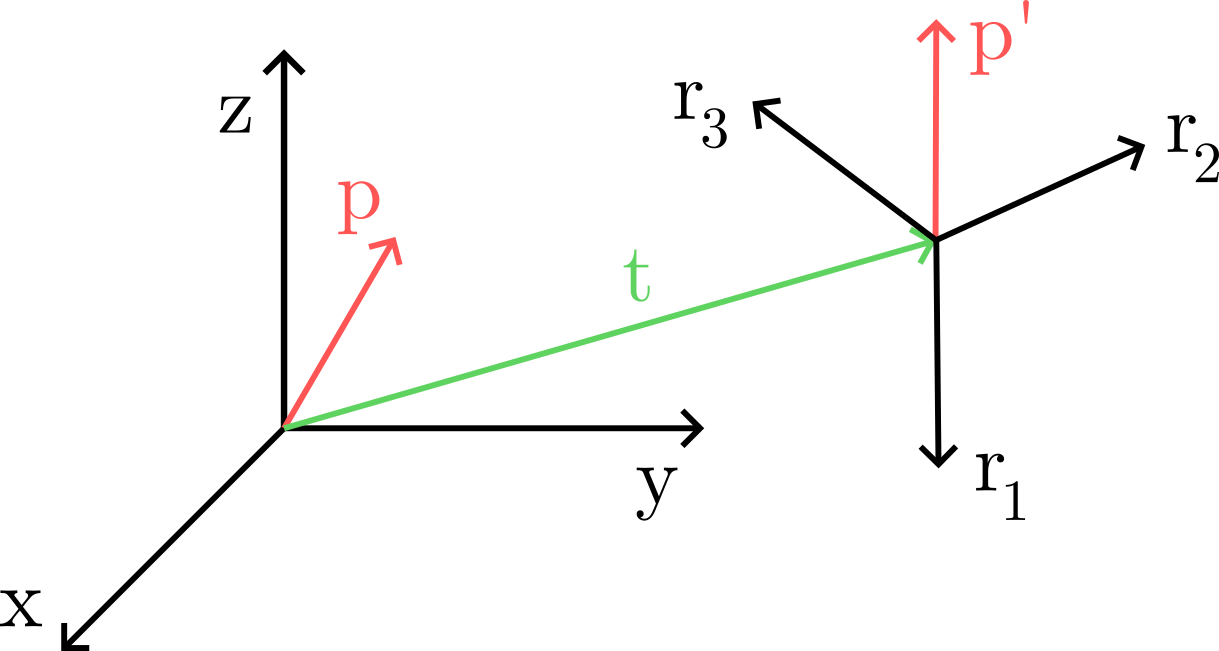
\includegraphics[scale=0.09]{../images/change-coords.png}
\end{minipage}%
\hfill
\begin{minipage}{0.5\textwidth} % Right side: Equation
    $
    p^{\prime} = 
    \underbrace{\left(
    \begin{array}{cccc}
    r_{\mathbf{1}} & r_{\mathbf{2}} & r_{\mathbf{3}} & t \\
    0 & 0 & 0 & 1
    \end{array}
    \right)}_{\mathbf{M}}
    \left(
    \begin{array}{c}
    p_x \\
    p_y \\
    p_z \\
    1
    \end{array}
    \right)
    $
\end{minipage}
Transforming a normal: $n^{\prime}=\left(\mathbf{M}^{-1}\right)^T n$, Alternatively: (rot(axis)) $\times$  (shift by $t$) 
}

\textbf{Projections}: $\mathbf{M}_{\mathrm{parallel}}= \operatorname{Diag}(1,1,0,1)$,$\mathbf{M}_{\mathrm{perspective}} = \left(
\begin{smallmatrix}
1 & 0 & 0  & 0 \\ 
0 & 1 & 0  & 0\\ 
0 & 0 & 1 & 0 \\
0 & 0 & \frac{1}{d} & 0 \\
\end{smallmatrix}
\right)$ where $d$ dist to camera (focal length)



\BDEF{Quaternions }{
Alternative approach for rotation. Similar to $\mathbb{C}$, define $i^2=j^2=k^2=-1, i j k=-1, i j=k$, $j i=-k, j k=i, k j=-i, k i=j, i k=-j$. For $q=a+$ $b i+c j+d k$, we have
\begin{itemize}[leftmargin = *,noitemsep]
\item $\|q\|=\sqrt{a^2+b^2+c^2+d^2}$
\item $\bar{z}=a-b i-c j-d k$ and $z^{-1}=\bar{z} /\|z\|$
\end{itemize}
Advantage: Efficient impl., Easy interpol., No Gimbal Lock

}

\BCODE{Rotation by Quaternions}{
Rotating a point $p=\left(\begin{array}{lll}x & y & z\end{array}\right)^T$ around axis $u=$ $\left(\begin{array}{lll}u_1 & u_2 & u_3\end{array}\right)$ by angle $\theta$.

\begin{enumerate} [leftmargin = *,noitemsep]
\item Convert $p$ to quaternion $p_Q=x i+y j+z k$
\item Convert $q$ to quaternion $q^{\prime \prime}=u_1 i+u_2 j+u_3 k$, normalize $q^{\prime}=q^{\prime \prime} /\left\|q^{\prime \prime}\right\|$
\item Rotate quaternion $q=\cos \frac{\theta}{2}+q^{\prime} \sin \frac{\theta}{2}$ and $q^{-1}=$ $\cos \frac{\theta}{2}-q^{\prime} \sin \frac{\theta}{2}$
\item Rotated point $p^{\prime}=q p q^{-1}$. Convert to cartesian.
\end{enumerate}


}

\mysubsection{2.4 Lighting \& Shading}
\textbf{Lighting}: Modelling physical interactions between materials and light sources\\
\textbf{Shading}: Process of determining color of pixel\\
\textbf{Solid angle}: $\Omega=\frac{A}{r^2}$ steradians (where $r$ radius)\\
\textbf{Zenith, Azimuth}: Point $\omega=(\theta, \phi)$ on unit sphere:

$
\omega_x=\sin \theta \cos \phi, \omega_y=\sin \theta \sin \phi, \omega_z=\cos \theta
$


\textbf{Energy of photon}: $\frac{h c}{\lambda}  \left [ J = \frac{\operatorname{kg} \operatorname{m^2}}{\operatorname{s}^2}\right ]$

\BDEF{Basic quanitities of radiometry}{

\textbf{Flux}: $\Phi(A)$ total amount of energy passing through surface or space per unit time $\left[\frac{\mathrm{J}}{\mathrm{s}}=\mathrm{W}\right]$\\
\textbf{Luminous flux}: $\int P(\lambda) V(\lambda) \mathrm{d} \lambda$. Perceived power of light weighted by human sensitiv. [lumen]\\ \textbf{Irradiance}: $E(x)=\frac{\mathrm{d} \Phi(A)}{\mathrm{d} A(x)}$ flux per unit area arriving at surface $\left[\frac{\mathrm{W}}{\mathrm{m}^2}\right]$.
\\ \textbf{Radiosity}: $B(x)=\frac{\mathrm{d} \Phi(A)}{\mathrm{d} A(x)}$ flux per unit area leaving a surface $\left[\frac{\mathrm{W}}{\mathrm{m}^2}\right]$
\\ \textbf{Radient / Luminous Intensity}: $I(\vec{\omega})=\frac{\mathrm{d} \Phi}{\mathrm{d} \vec{\omega}}$ outgoing
flux per solid angle $\left[\frac{\mathrm{W}}{\mathrm{sr}}\right] . \Phi=\int_{S^2} I(\vec{\omega}) \mathrm{d} \vec{\omega}$
\\ \textbf{Radiance}: $L(x, \vec{\omega})=\frac{\mathrm{d} I(\vec{\omega})}{\mathrm{d} A(x)}=\frac{S^2 \mathrm{~d}^2 \Phi(A)}{\mathrm{d} \overrightarrow{\mathrm{d}} \mathrm{d} A(x) \cos \theta}$ flux per solid angle per perp. area = intensity per unit area
}

\textbf{Lamberts cosine law}: Irradiance at surface is proportional to cosine of angle of incident light and surface normal: $E=(\Phi / A) \cos \theta$\\
\textbf{Bidir. reflectance distr. func. (BRDF)}: relation between incident radiance and diff. refl. radiance.

$$
f_r\left(x, \vec{\omega}_i, \vec{\omega}_r\right)=\frac{\mathrm{d} L_r\left(x, \vec{\omega}_r\right)}{\mathrm{d} E_i\left(x \vec{\omega}_i\right)}=\frac{\mathrm{d} L_r\left(x, \vec{\omega}_r\right)}{L_i\left(x, \vec{\omega}_i\right) \cos \theta_i \mathrm{~d} \vec{\omega}_i}
$$


\textbf{Reflection equation}: reflected radiance due to incident illumination from all directions (from BRDF): $\int_{H^2} f_r\left(x, \vec{\omega}_i, \vec{\omega}_r\right) L_i\left(x, \vec{\omega}_i\right) \cos \theta_i d \vec{\omega}_i=L_r\left(x, \vec{\omega}_r\right)$\\
\textbf{Types of reflections}: asc.  in comp. complexity with $\operatorname{BRDF}=f_r$:
\begin{enumerate}[leftmargin = *,noitemsep]
\item \textbf{Ideal Diffuse}: $f_r = c$ 
\item \textbf{Specular (Mirror)}: $f_r\left(\vec{\omega}_i, \vec{\omega}_r\right)=\delta\left(\vec{\omega}_r-\operatorname{reflect}\left(\vec{\omega}_i\right)\right)$
\item \textbf{Retro-reflective}:$f_r$ depends on $\vec{\omega}_i$,$\vec{\omega}_r$  but highly directional 
\item \textbf{Glossy Specular}: $f_r$ depends on $\vec{\omega}_i$,$\vec{\omega}_r$ 
\end{enumerate}
\textbf{Attenuation}: $f_{\text {att }}=\frac{1}{d_L^2}$ due to spatial radiation. Used in OpenGL: $f_{a t t}=\min \left(\frac{1}{c_1+c_2 d_L+c_3 d_L^2}, 1\right)$

\BDEF{Phong Illumination Model}{
Approximate specular reflection by cosine powers

$$
I_\lambda=\underbrace{I_{a_\lambda} k_a O_{d_\lambda}}_{\text {Ambient }}+f_{\text {att }} I_{p_\lambda}[\underbrace{k_d O_{d_\lambda}(\mathbf{N} \cdot \mathbf{L})}_{\text {Diffuse }}+\underbrace{k_s \overbrace{(\mathbf{R} \cdot \mathbf{V})^n}^{\approx \cos^n \beta}}_{\text {Specular}}]
$$

\begin{itemize}[leftmargin = *,noitemsep]
\item $I_\lambda$: reflected intensity for $\lambda$
\item $I_{a \lambda}$: Intensity of ambient light at $\lambda$
\item $k_a, 0 \leq k_a \leq 1$ Ambient reflection coefficient
\item $O_{d_\lambda}$ Object diffuse color at $\lambda$
\item $f_{\text {att }}$: Attenuation factor, accounts for light intensity reduction with dist.
\item $I_{p_\lambda}$: Intensity of the point light source at $\lambda$
\item $k_d, 0 \leq k_d \leq 1$ : Diffuse reflection coefficient, Controls how much of the incident light is diffusely reflected by the surface
\item $\mathbf{N}\in \mathbb{R}^{3}$: Surface normal
\item $\mathbf{L} \in \mathbb{R}^{3}$: Direction from the surface point to the light source 
\item $k_s,0 \leq k_s \leq 1$: Specular reflection coefficient, controls shininess of the surface
\item $\mathbf{R}\in \mathbb{R}^{3}$: Reflected light direction 
\item $\mathbf{V}\in \mathbb{R}^{3}$: Viewing direction
\end{itemize}

}
\textbf{Extension}: Can be extended to multiple sources of light: $I_{a_\lambda} k_a+\sum_{1 \leq i \leq m} f_{a t t_i} I_{p_{\lambda_i}}\left[k_d\left(\mathbf{N} \cdot \mathbf{L}_i\right)+k_s\left(\mathbf{R}_i \cdot \mathbf{V}\right)^n\right]$ and made faster with half-way vector: $(\mathbf{N} \cdot \mathbf{H})^n$ where $\mathbf{H}=\frac{\mathbf{L}+\mathbf{V}}{\|\mathbf{L}+\mathbf{V}\|}$ 

\mysubsection{2.5 Shading Models}
\textbf{Flat Shading (Screen Space)}: one color per primitive, works when light-sources is at inf. or primitive is very small.

\BCODE{Gouraud Shading (Screen Space) }{
Lin.interpol. vertex intensities
\begin{enumerate}[leftmargin = *,noitemsep]
\item \textbf{Calculate face normals}
\item \textbf{Calculate vertex normals}: For each vertex $v$ compute $N_v=\left( \sum_{i=1} N_i \right)
\left( \left|\sum_{i=1}^N N_i\right|\right)^{-1}$, $N_i$ are adjacent normals to $V$
\item \textbf{Evaluate illumination model}: For each vertex
\item \textbf{Interpolate vertex colors}: Bilinearly on the current scan line

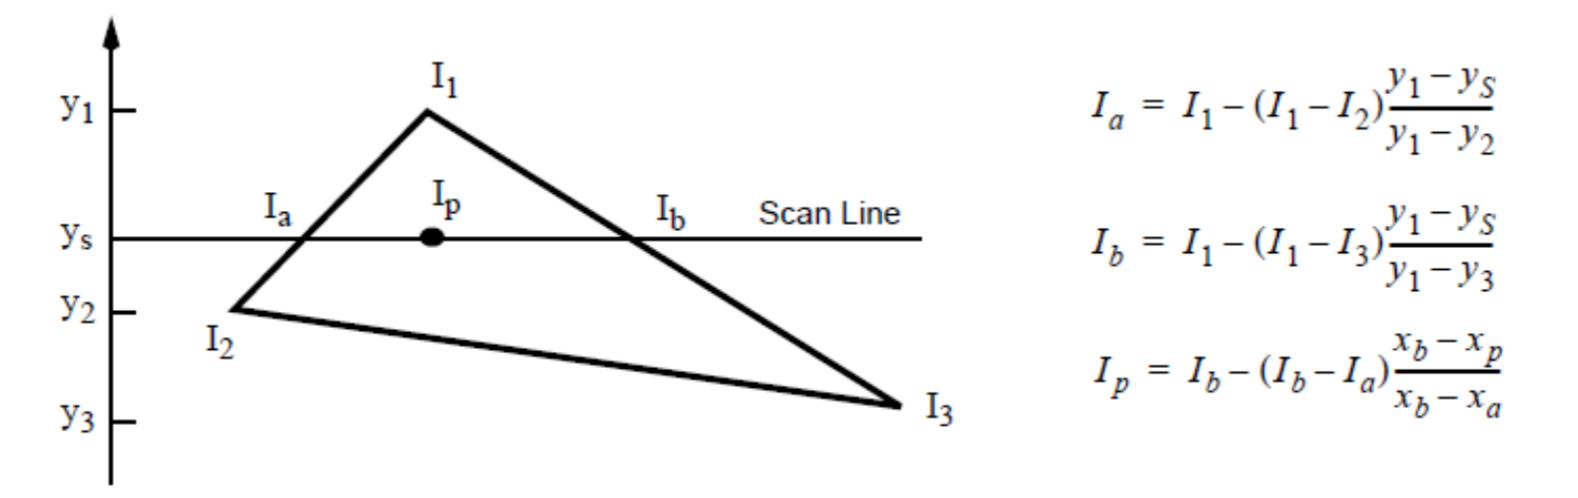
\includegraphics[width=\linewidth]{../images/scan_line.png} 

\end{enumerate}

Problems with scan line interpolation are perspective distortion, orientation dependence, shared vertices. Quality depends on size of primitives.

}

\BCODE{Phong Shading (Object Space)}{

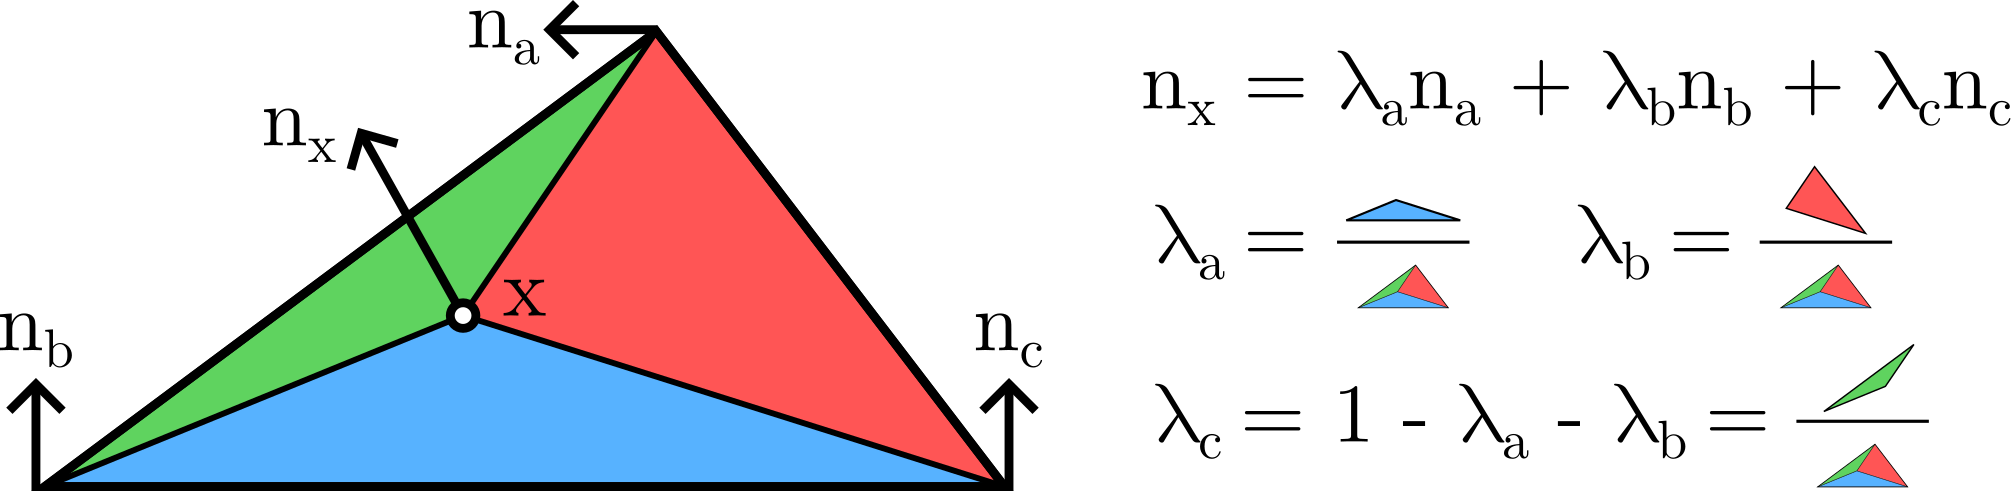
\includegraphics[width=\linewidth]{../images/phong-shading.png} 

\textbf{Properties}: Lagrange: $x=a \Rightarrow n_x=n_a$ \\
\textbf{Partition of unity}: $\lambda_a+\lambda_b+\lambda_c=1$ \\
\textbf{Reproduction}: $\lambda_a \cdot a+\lambda_b \cdot b+\lambda_c \cdot c=x$. \\
\textbf{Problems}: normal not defined / representative.
}
\textbf{$\mathbf{\alpha}$-blending}: Achieves simple transparency. Perceived intensity $I_\lambda=I_{\lambda_1}^{\prime}+I_{\lambda_2}^{\prime}$ where $I_{\lambda_1}^{\prime}$ is emission of $P_1$ and $I_{\lambda_2}^{\prime}$ is intensity filtered by $P_1$. We model it as follows: $I_\lambda=$ $I_{\lambda_1} \alpha_1 \Delta t+I_{\lambda_2} e^{-\alpha_1 \Delta t}$ where $\alpha$ absorption, $\Delta t$ thickness.



\\ \textbf{Linearization}: 



\begin{multicols}{2}
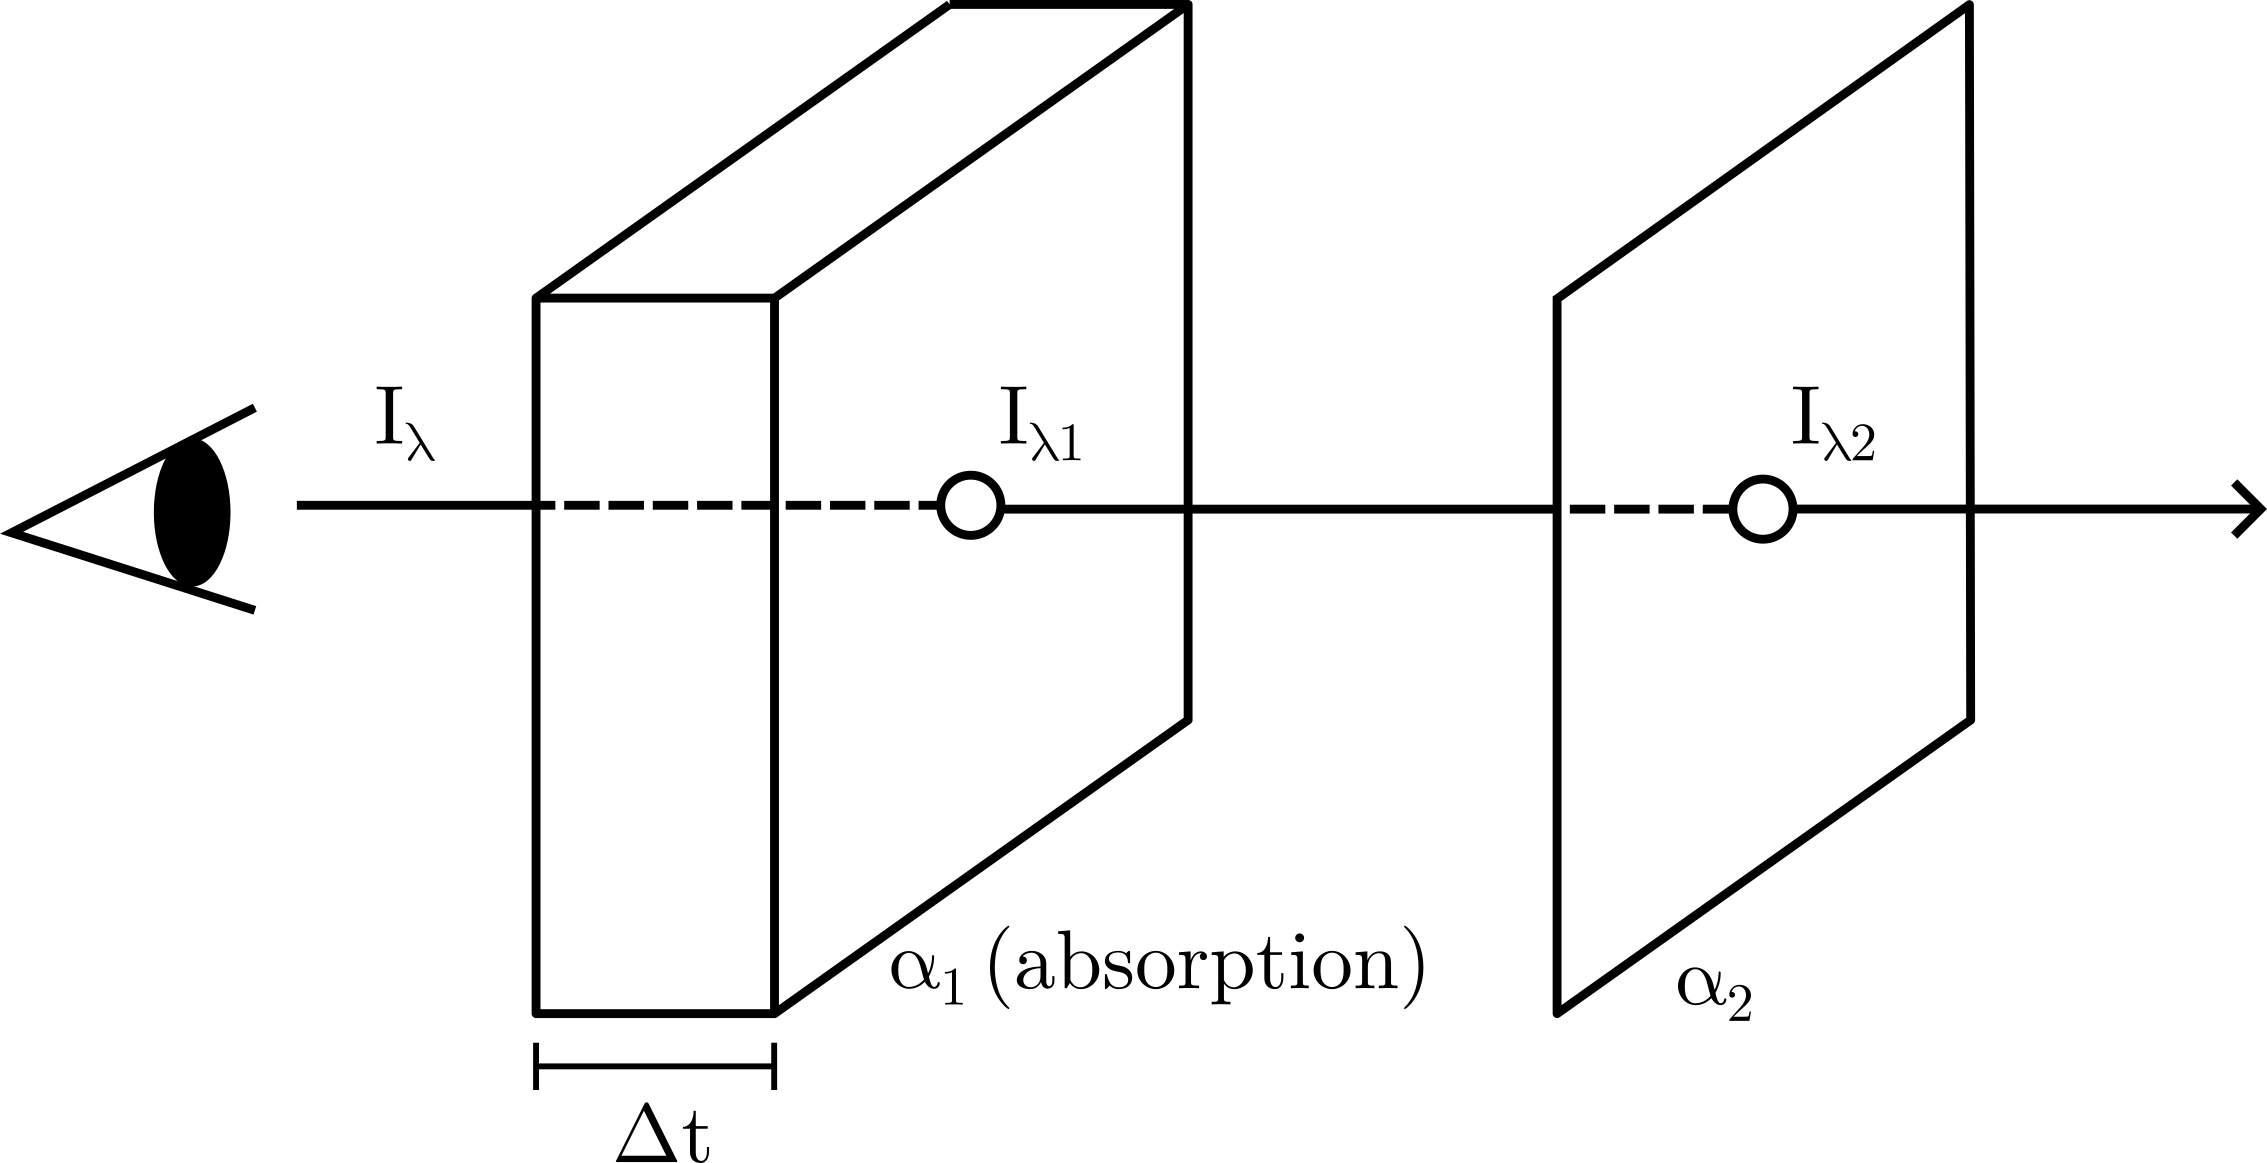
\includegraphics[width=\linewidth]{../images/transparency.png}

\columnbreak
$I_\lambda=I_{\lambda_1} \alpha_1 \Delta t+I_{\lambda_2}\left(1-\alpha_1 \Delta t\right)$. If last object, set $\Delta t=1$. Problem: rendering order, sorted traversal of polygons and back-to-front rendering.

\end{multicols}
Back-to-front order not always clear, resort to depth peeling, multiple passes, each pass renders next closest fragment. We need more advanced lighting models for metal objects (Cook-Torrence), replacing specular term, with reflection from micro facets, self-shadowing... 

\mysubsection{2.6 Geometry \& Textures}

\textbf{Considerations}: Storage, acquisition of shapes, creation of shapes, editing shapes, rendering shapes. Explicit repr. can easily model complex shapes, and sample points, but take lots of storage.
\begin{itemize}[leftmargin = *,noitemsep]
\item \textbf{Subdivision surface}: Define surfaces by primitives, use recursive algorithm for refining
\item \textbf{Point set surfaces}: Store points as surface
\item \textbf{Polygonal meshes}: Explicit set of vertices with position, possibly with additional information. Intersection of polygons: either empty, vertex, edge.
\end{itemize}


Implicit repr. easily test inside / outside, compact storage, but sampling expensive, hard to model
\textbf{Implicit surfaces}: surface = zeros of a function

We need to store textures as bitmaps, hence parameterizing complex surfaces.

\textbf{Manifolds}: surface homeomorphic to disk, (1) most 2 faces share an edge, (2) conn. (half-)ring of faces\\

\textbf{Mesh data structures}: Locations, how vertices are connected, attributes such as normals, color etc. Must support rendering, geometry queries, modifications. E.g.
 \begin{itemize}[leftmargin = *,noitemsep]
\item Triangle list (list of 3 points, redundant, e.g. STL).
\item Indexed Face set (array of vertices + list of indices, e.g. OBJ, OFF, WRL, costly queries, modifications)
 \end{itemize}

\textbf{Bandlimiting}: Restrict amplitude of spectrum to zero for frequency beyond cut-off frequency.

\textbf{Anti-aliasing filters}:

\begin{itemize}[leftmargin = *,noitemsep]
\item Gaussian (low-pass, separable). Closer pixels have higher weight
\item Sinc $S_{\omega_c}(x, y)=\frac{\omega_c \operatorname{sinc}\left(\frac{\omega_c x}{\pi}\right)}{\pi} \times \frac{\omega_c \operatorname{sinc}\left(\frac{\omega_c y}{\pi}\right)}{\pi}$ ideal lowpass filter, IIR filter. $\omega_c$ cutoff freq. Hard to implement, has infinite impulse respons.
\item B-Spline: Allow for locally adaptive smoothing, adapt size of kernel to signal chars. 
\end{itemize}


\textbf{Magnification}: for pixels mapping to area larger than pixel (jaggies), use bilinear interpolation. \\

\textbf{Mipmapping}: Store texture at multiple resolutions, choose based on projected size of triangle (far away $\rightarrow$ lower res, interpol. possible). Avoids aliasing, improves efficiency, higher storage overhead. (minification) \\

\textbf{Supersampling}: Multiple color samples per pixel, final color is average - different patterns of samples possible (uniform, jittering, stochastic, Poisson). \\

\textbf{Light map}: Simulate effect of local light source. Can be pre-computed and dynamically adapted
Environment map: Mirror environment with imaginary sphere or cube for reflective objects \\
\textbf{Bump map}: Perturb surface normal according to texture, represents small-scale geometry. Limitations: no bumps on silhouette, no self-occlusions, no self-shadowing. Height stored as grayscale textures. \\

\textbf{Procedural texture}: Generate texture from noise (Perlin, Gabor) from Guassian pyramid of noise and summing layers with weights.\\

\textbf{Perspective interpolation} in world-space can yield non-linear variation in screen-space. Optimal resampling filter is hence spatially variant.

\mysubsection{2.7 Scan Conversion}

Generate discrete pixel values - approxiate with finit amount.\\
\textbf{Bresenham line}: choose closest pixel at each intersection. Fast decision, criterion based on midpoint $m$ and intersection point $q$. After computing first value $d$, we only need addition, bitshifts. $d_{\text {new }}=d_{\text {old }}+a$

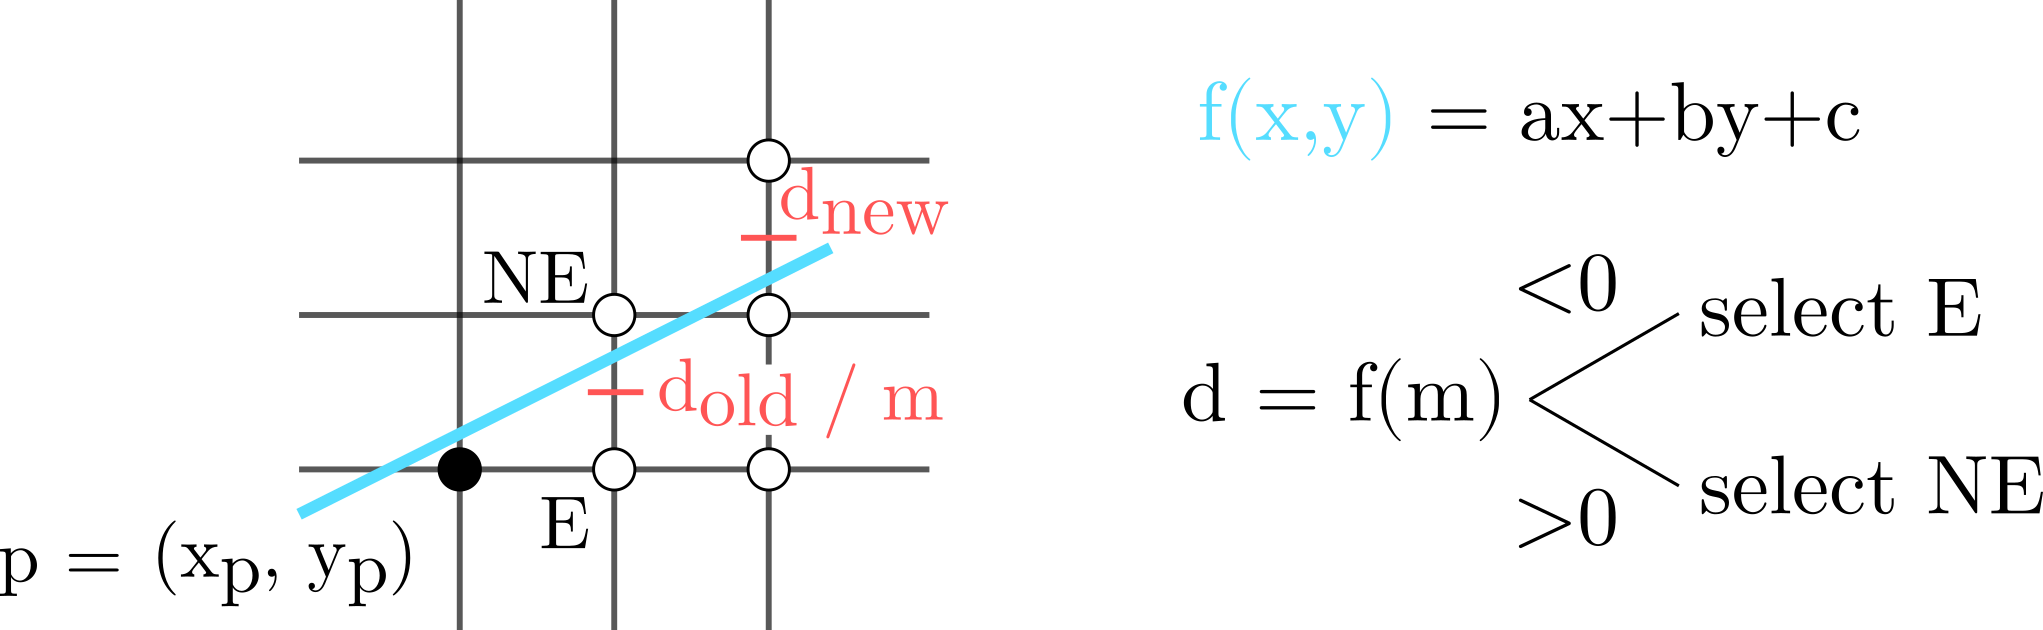
\includegraphics[width = \linewidth]{../images/bresenham-line.png} 

\textbf{Implementation}: \textcolor{col1}{def bhmline(x0, y0, x1, y1):}\textcolor{col2}{dx = x1 - x0;dy = y1 - y0;d = 2 * dy - dx;}\textcolor{col2}{incE = 2 * dy;incNE = 2 * (dy - dx);x = x0;y = y0;writepixels(x, y);}\textcolor{col3}{while x < x1:}
\textcolor{col4}{if d $\leq$ 0:}\textcolor{col5}{d += incE;}\textcolor{col4}{else:} \textcolor{col5}{d += incNE;y += 1;}\textcolor{col4}{        x += 1;writepixels(x, y);}

Scan conversion of polygons:\begin{enumerate}[leftmargin = *,noitemsep]
\item Calculate intersections on scan line
\item  Sort intersection points by ascending $x$-coords.
\item Fill spans between two consecutive intersection points if parity in interval is odd (so inside)
\end{enumerate} 
\textbf{Implementation}:
\textcolor{col1}{def leftedgescan(xmin, ymin, xmax, ymax):}\textcolor{col2}{x = xmin;;num = xmax - xmin;denom = ymax - ymin;}\textcolor{col2}{inc = denom;for y in range(ymin, ymax + 1):}
\textcolor{col3}{write_pixels(x, y);inc += num;if inc > denom:}\textcolor{col4}{x += 1;inc -= denom}





\mysubsection{2.8 Bézier Curves \& Splines}

\textbf{Disadvantages of Bézier}: global support of basis functions, new control pts yields higher degree, $C^n$ continuity between segments of Bézier-Curves, imposes constraints. 
$C^{1}$: $P_n^{(i)}=P_0^{(i+1)}$ ,$C^{2}$: $P_{n-1}^{(i)}-P_n^{(i)}=k \cdot\left(P_1^{(i+1)}-P_0^{(i+1)}\right)$
\BDEF{Bézier Curves}{

$\boldsymbol{x}(t)=\boldsymbol{b}_0 B_0^n(t)+\ldots+\boldsymbol{b}_n B_n^n(t)$ where $B_i^n$ are the Bernstein polyn. $\left(\binom{n}{i}=\frac{n!}{i!(n-i)!}\right)$ : $B_i^n(t)=\binom{n}{i} t^i(1-t)^{n-i}$ if $i \neq 0$ else 0 (partition of unity, pos. definite, recursion, symmetry). Coefficients $b_0, \ldots, b_n$ are called control- / Bézier-points, together define the control polygon.

Degree is highest order of polyn., order is deg. + 1. Bézier-Curves have affine invariance (affine transf. of curve accompl. by affine transf. of control pts.). Curve lies in convex hull of control polygon $\operatorname{conv}(P):=\left\{\sum_{i=1}^n \lambda_i \boldsymbol{p}_i \mid \lambda_i \geq 0, \sum_{i=1}^n \lambda_i=1\right\}$. Control polyg. gives rough sketch of curve. Since $B_0^n(0)=$ $B_n^n(1)=1$, interpol. endpoints $b_0, \boldsymbol{b}_n$. Max. number of intersect. of line with curve is $\leq$ number of intersect. with control polygon. Bézier curves are special cases of B-spline curves. 
}



\BDEF{B-Spline functions }{B-Spline curve $s(u)$ built from piecewise polyn. bases $s(u)=\sum_{i=0}^k \boldsymbol{d}_i N_i^n(u)$
Coefficients $\boldsymbol{d}_i$ are called "de Boor" pts. Bases are piecewise, recursively def. polyn. over sequence of knots $u_0<u_1<u_2<\ldots$ defined by knot vec. $T=\boldsymbol{u}=$ $\left(u_0 \ldots u_{k+n+1}\right)$
Partition of unity $\sum_i N_i^n(u) \equiv 1$, positivity $N_i^{n(u)} \geq$ 0 , compact support $N_i^{n(u)}=0, \forall u \notin\left[u_i, u_{i+n+1}\right]$, continuity $N_i^n$ is $(n-1)$ times cont. differentiable.}
\textbf{deCasteljau}: Compute a triangular representation, successively interpolate, "corner cutting" with control points $ b_0, b_1, b_2$\\
\begin{minipage}{0.20\linewidth} 
$\begin{array}{llll}b_0 & & & \\ b_1 & b_0^1 & & \\ b_2 & b_1^1 & b_0^2 & \\ b_3 & b_2^1 & b_1^2 & b_0^3\end{array}$
\end{minipage}
\hfill
\begin{minipage}{0.75\linewidth} 
$$
\begin{aligned}
& b_0^1(t)=(1-t) b_0+t b_1 \\
& b_1^1(t)=(1-t) b_1+t b_2 \\
& b_0^2(t)=(1-t) b_0^1(t)+t b_1^1(t)
\end{aligned}
$$

\end{minipage}

\textbf{deBoor}: generalizes deCasteljau, evaluate Bspline of degree $n$ at $u$, set $d_i^0=d_i$, finally $d_0^n=s(u)$

$
d_i^k=\left(1-a_i^k\right) d_i^{k-1}+a_i^k d_{i+1}^{k-1}, \quad a_i^k=\frac{u-u_{i+k-1}}{u_{i+n}-u_{i+k-1}}
$
$a_i^k$ vanishes outside of $\left[\boldsymbol{u}_{i+k-1}, u_{i+n}\right]$ 

\textbf{Implementation}:
\textcolor{col1}{def deBoor(k: int, x: int, t, c, p: int):}\textcolor{col2}{d = [c[j + k - p] for j in range(0, p + 1)];for r in range(1, p + 1):}\textcolor{col3}{ for j in range(p, r - 1, -1):}\textcolor{col4}{alpha = (x - t[j + k - p]) / (t[j + 1 + k - r] - t[j + k - p]);d[j] = (1.0 - alpha) * d[j - 1] + alpha * d[j];}\textcolor{col2}{return d[p]}
 
\mysubsection{2.9 Subdivision Surfaces}
Generalization of spline curves / surfaces allowing arbitrary control meshes using successive refinement (subdivision), converging to smooth limit surfaces, connecting splines and meshes.

\begin{minipage}{0.25\linewidth} % Image column (1/8 of the width)
    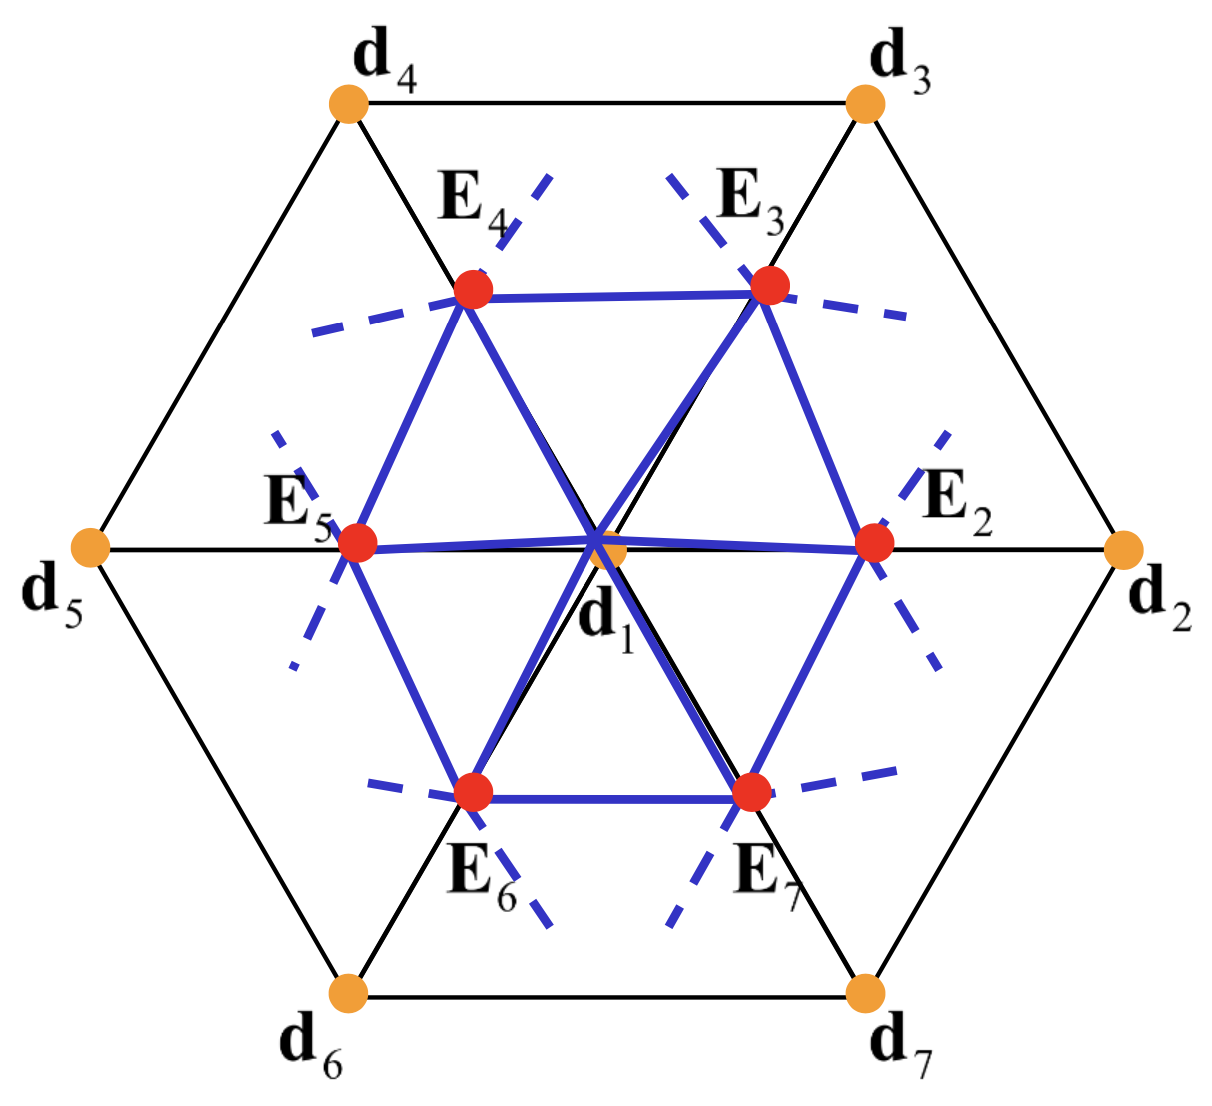
\includegraphics[width=\linewidth]{../images/loop-subdivision.png} 
\end{minipage}
\hfill
\begin{minipage}{0.70\linewidth} % Text column (7/8 of the width)
    \textbf{Loop Subdivision}:

$E_i=\left(\frac{3}{8}\right) \cdot\left(d_1+d_i\right)+\left(\frac{1}{8}\right) \cdot\left(d_{i-1}+d_{i+1}\right)$

$d_{1^{\prime}}=\alpha_n \cdot d_1+\frac{1-\alpha_n}{n} \cdot \sum_{j=2}^{n+1}\left(d_j\right)$

$\alpha_n=\frac{3}{8}+\left(\frac{3}{8}+\frac{1}{4 n} \cos (2 \pi)\right)^2$
\end{minipage}

\begin{minipage}{0.25\linewidth} % Image column (1/8 of the width)
\begin{center}
 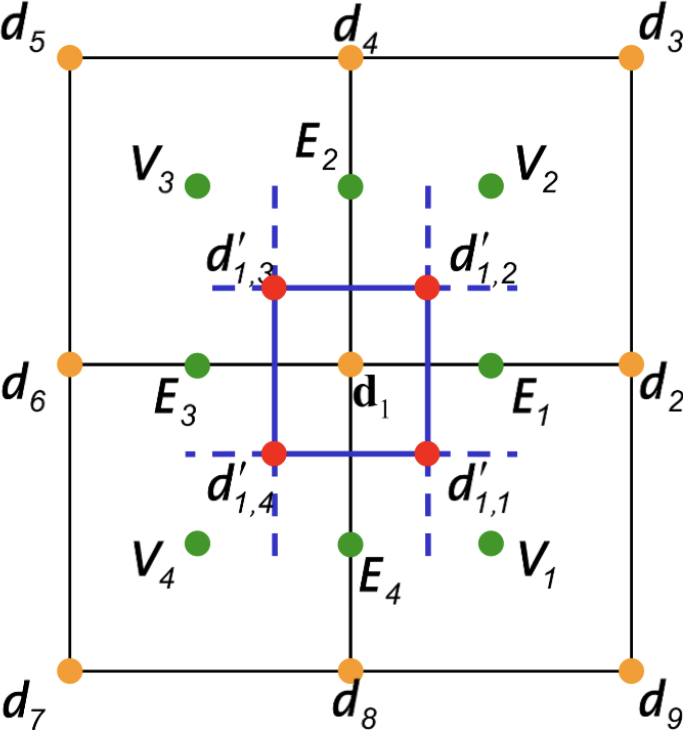
\includegraphics[width=0.8\linewidth]{../images/doo-sabin-subdivision.png}
\end{center}
   
\end{minipage}
\hfill
\begin{minipage}{0.70\linewidth} % Text column (7/8 of the width)

    \textbf{Doo-Sabin Subdivision}:\\
    $ V_2=\frac{1}{n} \sum_{j=1}^n d_j, E_i=\frac{1}{2}\left(d_1+d_{2 i}\right)$
$d_{(1, j)^{\prime}}=\frac{1}{4}\left(d_1+E_j+E_{j-1}+V_j\right)$
\end{minipage}

\textbf{Properties}: Both: Appr, Loop:primal, works on triangles,$C_1$ cont. (extra-ordinary points, valence $\neq 6$), $C_2$ cont. else  ;Doo-Sabin:dual, works on arbitrary polygon meshes, $C_1$ cont.,  

\textbf{Classification}: faces are split (\textbf{primal})vs vertcies are split (\textbf{dual}); new points are an interpolation of control points (\textbf{Interpolating}) vs controls points are moved, and new points are added inbetween (\textbf{Approximating})\\



\mysubsection{2.10 Visibility \& Shadows}
\textbf{Scan Line Shadow Calculation}: The edges of possibly shadow-casting polygons are projected onto all polygons in the direction of the light flux that are intersected by the current scan line. $\mathcal{O}(n^2)$
\textbf{Painter's algorithm}: Render objects from furthest to nearest. Issues with cyclic overlaps \& intersec.\\
\textbf{Z-Buffer}: store depth to nearest obj for each px. Initialize to $\infty$, then iter. over polygons and update z-buffer. Limited resolution, non-linear, place far from camera Planar shadows: draw projection of obj. on ground. No self-shadows, no shadows on other objects, curved surfaces.\\
\textbf{Projective texture shadows}: Separate obstacles and receivers, compute $\mathrm{b} / \mathrm{w}$ img. of of obst. from light, use as projective textrue. Need to specify obstacle \& receiver, no self-shadows.

\BDEF{Shadow maps }{Compute depths from light \& camera. For each px on camera plane, compute point in world coords., project onto light plane, compare $d\left(\boldsymbol{x}_L\right)$ (dist. from light source to projected point on light plane) to $z_L$ (dist light source to $x_L$ ). If $d\left(\boldsymbol{x}_L\right)<z_L$, then $x$ in shadow. Bias needed to avoid self-shadowing $\left(d\left(x_L\right)+\right.$ $b<z_L$ ). Point to shadow can be outside field of view of (use cubical shadow map or spot lights). Aliasing due to undersampling shadow map (filter result of depth test).}

\textbf{Shadow volumes}: Explicitly represent volume of space in shadow. If polygon in volume, it is in shadow. Shoot ray from camera, increment each time boundary of shadow volume is intersected. If counter $>0$, primitive is in shadow. Optimization: use silhouette edges only. Introduces a lot of new geometry, expensive to rasterize long skinny triangles. Objects must be watertight for silhouette optimizations. Rasterization of polygons must not overlap \& not have a gap.

\mysubsection{2.11 Ray Tracing}

\BDEF{Ray Tracing}{
Send rays into scene to determine color of px. On obj. hit, send mult. rays (diffused, reflected, refracted) further until we hit light source, or reach some amount of bounces. Figure out whether point in shadow by shooting rays to all light sources. For anti-aliasing, use mult. rays per px. (Pipel.: Ray Generation, Intersection, Shading)
}


\textbf{Ray-surface intersections}: Ray equation $\boldsymbol{r}(t)=\boldsymbol{o}+$ $t \boldsymbol{d}$. Sphere: $\|\boldsymbol{x}-\boldsymbol{c}\|-r^2=0$ where $\boldsymbol{x}$ point of interest, $\boldsymbol{c}$ center, $r$ radius. Solve for $t:\|\boldsymbol{o}+t \boldsymbol{d}-\boldsymbol{c}\|^2-r^2=0$. \\ \textbf{Triangle}: Barycentric coords. $\boldsymbol{x}=s_1 \boldsymbol{p}_1+s_2 \boldsymbol{p}_2+s_3 \boldsymbol{p}_3$. Intersect: $\left(\boldsymbol{o}+t \boldsymbol{d}-\boldsymbol{p}_1\right) \cdot n=0$. Using the following: $\boldsymbol{n}=\left(\boldsymbol{p}_2-\boldsymbol{p}_1\right) \times\left(\boldsymbol{p}_3-\boldsymbol{p}_1\right)$ we get $t=-\frac{\left(\boldsymbol{o}-\boldsymbol{p}_1\right) \cdot \boldsymbol{n}}{\boldsymbol{d} \cdot \boldsymbol{n}}$. Now compute the coeffs. $\boldsymbol{s}_i$. Test whether $s_1+s_2+s_3=1$ and $0 \leq s_i \leq 1$. If so, inside triangle.\\

\textbf{Ray-tracing shading extensions}: Refraction, mult. lights, area lights for soft shadows, motion blur (sample


objs, intersect in time), depth of field \\
\textbf{Cost}: $O\left(N_x N_y N_o\right)=\# \mathrm{px} \cdot \# \mathrm{objects}$ \\
\textbf{Accelerate}: Accelerate with less intersections, introduce uniform grids or space partitioning trees. \\
\textbf{Uniform grids}: Preprocess: compute bounding box, set grid res., rasterize objects, store refs. to objects. Traversal: incrementally rasterize rays - stop at intersection. Fast \& easy, but non-adaptive to scene geometry.\\
 \textbf{Space partitioning trees}: octree, kd-tree, bsp-tree

Another solution: bounding volume hierarchies (BVH)


\begin{enumerate}[leftmargin = *,noitemsep]
\item Grayscale images range from 0 (black) to 255 (white).
\item Frequency: High (rapid changes in intensity or color)
\item Quotient Role: $(f/g)'=(f'g-fg')/(g^2)$
\item (255) need one byte. Thus RGB need $3$ bytes per px
\item Butterfly (triangles, primal, interpol), Kobbelt (rect, primal, interpol), Catmull-Clark (rect, approx, primal)
\end{enumerate}


